%
%===============>>  Сорокин Модуль 7 <<=============
%
\setmodule{7}

%BEGIN_FOLD % ====>>_____ Занятие 1 _____<<====
\begin{class}[number=1]
	\begin{listofex}
		\item Решите неравенства:
		\begin{tasks}(2)
			\task \( \sqrt{x-3}<2 \)
			\task \( \sqrt{2x+1}>5 \)
			\task \( \sqrt{x+1}>-2 \)
			\task \( \sqrt{17x+6}<-1 \)
		\end{tasks}
		\item Решите неравенства:
		\begin{tasks}(2)
			\task \( \sqrt{2x^2-3x+2}\le-4 \)
			\task \( \sqrt{2x^2-3x+2}\ge4 \)
		\end{tasks}
		\item Решите неравенства:
		\begin{tasks}(2)
			\task \( \sqrt{x+8}<x+2 \)
			\task \( \sqrt{x-2}\le x-2 \)
			\task \( \sqrt{x+7}>x+3 \)
			\task \( \sqrt{x^2+2x}>-3-x^2 \)
		\end{tasks}
		\item Решите неравенства:
		\begin{tasks}(2)
			\task \( \sqrt[5]{x^2-12}>-2 \)
			\task \( (x^2-12)^{\tfrac{1}{5}}>-2 \)
		\end{tasks}
	\end{listofex}
\end{class}
%END_FOLD

%BEGIN_FOLD % ====>>_ Домашняя работа 1 _<<====
\begin{homework}[number=1]
	\begin{listofex}
		\item 
		\begin{tasks}
			\task \(  \)
			\task \(  \)
			\task \(  \)
			\task \(  \)
		\end{tasks}
	\end{listofex}
\end{homework}
%END_FOLD

%BEGIN_FOLD % ====>>_____ Занятие 2 _____<<====
\begin{class}[number=2]
	\begin{listofex}
		\item Решите неравенства: % 12-27 б
		\begin{tasks}(2)
			\task \( 7^{2x^2+3x}>49 \)
			\task \( 5^{x^2-6x+11} \le 25 \)
			\task \( 3^x \cdot 4^x  \le 144 \)
			\task \( 16^x \cdot 64^x \ge 0,25 \)
			\task \( 6^x < 9 \cdot 2^x \)
			\task \( 9^x \cdot 3^{x^2} \ge 27 \)
			\task \( 14^{x-16} \le 15^{x-16} \)
			\task \( 4^{7-4x} \ge 3^{4x-7} \)
			\task \( 13^{x^2-9}<14^{x^2-9} \)
			\task \( 5^{25-4x^2}>2^{4x^2-25} \)
			\task \( 4 \cdot 9^{x-8} \le 9 \cdot 4^{x-8} \)
			\task \( 16 \cdot 5^{x-8} \ge 25 \cdot 4^{x-8} \)
			\task \( 64 \le \dfrac{ 1 }{ 4^{2x+9} } \)
			\task \( 3^{4x^2-13x}>\dfrac{ 1 }{ 27 } \)
			%\task \( (\sqrt[5]{17})^{10x} \le \sqrt{17} \)
			%\task \( \sqrt[7]{13^x}<169 \)
		\end{tasks}
		\item Решите неравенства:
		\begin{tasks}(2)
			\task \( \sqrt[6]{4x-x^2-3}<1 \)
			\task \( \sqrt[4]{x^2-4x+85}\le 3 \)
		\end{tasks}
	\end{listofex}
\end{class}
%END_FOLD
%BEGIN_FOLD % ====>>_____ Занятие 3 _____<<====
\begin{class}[number=3]
	\begin{listofex}
		%11.1v2v3 po 4-7
		\item Найдите точку максимума функции \( y=x^3-3x^2+2 \).
		\item Найдите точку минимума функции \( y=2x^3-5x^2+25 \).
		\item Найдите наименьшее значение функции \(y=x^3-3x^2+2\) на отрезке \( [1;4] \).
		\item Найдите наибольшее значение функции \(y=x^3-6x^2\) на отрезке \( [-3;3] \).
		
		%5-8 analog 282861
		\item Найдите наименьшее значение функции \( y=(x-3)^2(x-6)-1 \) на отрезке \( [4;6] \).
		\item Найдите наименьшее значение функции \( y=(x-6)^2(x+4)-3 \) на отрезке \( [1;11] \).
		\item Найдите наименьшее значение функции \( y=(x-7)^2(x-6)+6 \) на отрезке \( [6,5;19] \).
		\item Найдите наименьшее значение функции \( y=(x-10)^2(x+4)+7 \) на отрезке \( [2;14] \).
		
		\item Найдите наибольшее значение функции \( y=\dfrac{ x^2+25 }{ x } \) на отрезке \( [-10;-1] \).
		\item Найдите точку максимума функции \( y=\dfrac{ 16 }{ x }+x+3 \).
		\item Найдите минимума функции функции \( y=\dfrac{ 25 }{ x }+x+25 \).
		\item Найдите наименьшее значение функции \( y=x+\dfrac{ 36 }{ x } \) на отрезке \( [1;9] \).
		
		\item Найдите точку минимума функции \( y=(3-x)e^{3-x} \).
		\item Найдите точку максимума функции \( y=(x+16)e^{16-x} \).
		\item Найдите точку минимума функции \( y=(3x^2-36x+36)e^{x-36} \).
		\item Найдите точку максимума функции \( y=(x^2-12x+12)e^{x+12} \).
		
		
		
		%G111M5L2
		\item
		\begin{minipage}[t]{\bodywidth}
			На рисунке изображен график функции \( y = f(x)\), определенной на интервале \((-5; 5)\). Найдите количество точек, в которых касательная к графику функции параллельна прямой \(y  =  6\) или совпадает с ней.
		\end{minipage}
		\hspace{0.02\linewidth}
		\begin{minipage}[t]{\picwidth}
			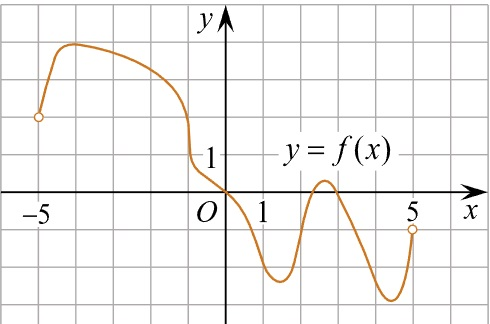
\includegraphics[align=t, width=\linewidth]{../\picpath/G111M5L2-1}
		\end{minipage}
		\item
		\begin{minipage}[t]{\bodywidth}
			На рисунке изображен график производной функции \(f(x)\), определенной на интервале \((-10; 2)\). Найдите количество точек, в которых касательная к графику функции \(f(x)\) параллельна прямой \(y = -2x - 11\) или совпадает с ней.
		\end{minipage}
		\hspace{0.02\linewidth}
		\begin{minipage}[t]{\picwidth}
			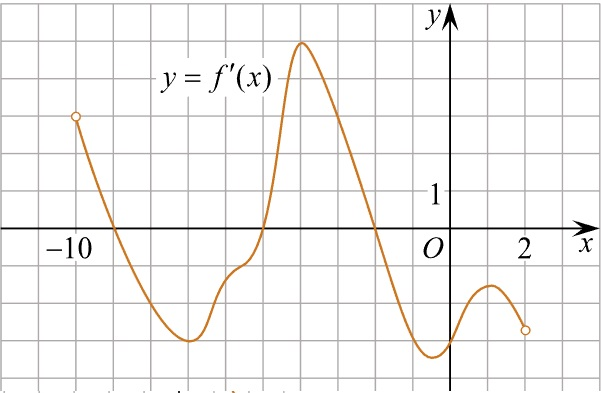
\includegraphics[align=t, width=\linewidth]{../\picpath/G111M5L2-2}
		\end{minipage}
		%541816
		\item
		\begin{minipage}[t]{\bodywidth}
			На рисунке изображены график функции \(y=f(x)\) и касательная к нему в точке с абсциссой \(x_0\). Найдите значение производной функции \(f(x)\)в точке \(x_0\).
		\end{minipage}
		\hspace{0.02\linewidth}
		\begin{minipage}[t]{\picwidth}
			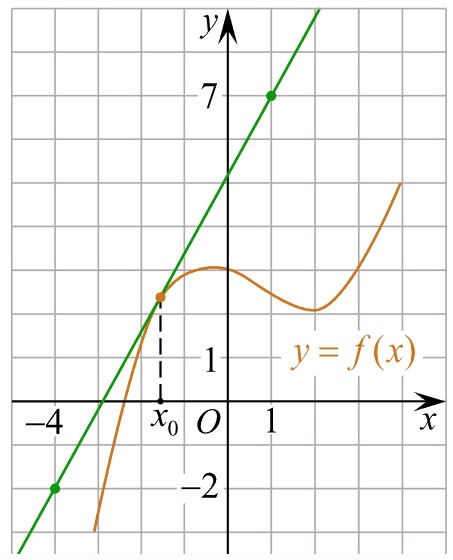
\includegraphics[align=t, width=\linewidth]{../\picpath/maksutovM8L4-1}
		\end{minipage}
		%9063
		\item
		\begin{minipage}[t]{\bodywidth}
			На рисунке изображены график функции \(y=f(x)\) и касательная к нему в точке с абсциссой \(x_0\). Найдите значение производной функции \(f(x)\)в точке \(x_0\).
		\end{minipage}
		\hspace{0.02\linewidth}
		\begin{minipage}[t]{\picwidth}
			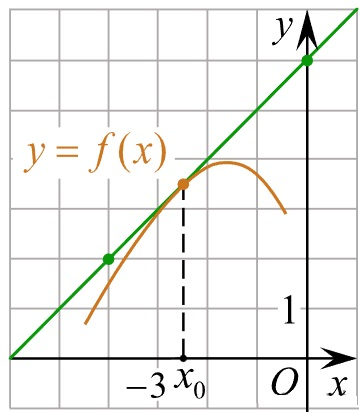
\includegraphics[align=t, width=\linewidth]{../\picpath/maksutovM8L4-2}
		\end{minipage}
		%9629
		\item
		\begin{minipage}[t]{\bodywidth}
			На рисунке изображены график функции \(y=f(x)\) и касательная к нему в точке с абсциссой \(x_0\). Найдите значение производной функции \(f(x)\)в точке \(x_0\).
		\end{minipage}
		\hspace{0.02\linewidth}
		\begin{minipage}[t]{\picwidth}
			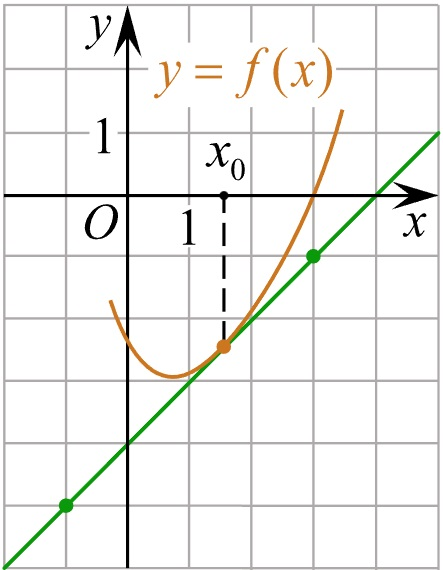
\includegraphics[align=t, width=\linewidth]{../\picpath/maksutovM8L4-3}
		\end{minipage}
	\end{listofex}
\end{class}
%END_FOLD

%BEGIN_FOLD % ====>>_ Домашняя работа 3 _<<====
\begin{homework}[number=3]
	\begin{listofex}
		\item Домашняя работа
	\end{listofex}
\end{homework}
%END_FOLD

%BEGIN_FOLD % ====>>_____ Занятие 4 _____<<====
\begin{class}[number=4]
	\begin{listofex}
		\item 
		\begin{minipage}[t]{\bodywidth}
			На рисунке изображён график функции \(f(x)=kx+b\). Найдите \(f(-5)\).
		\end{minipage}
		\begin{minipage}[t]{\picwidth}
			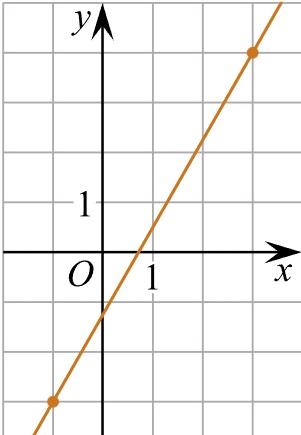
\includegraphics[align=t, width=0.8\textwidth]{../\picpath/G101M4H2-1.jpg}
		\end{minipage}
		\item
		\begin{minipage}[t]{\bodywidth}
			На рисунке изображены графики двух линейных функций. Найдите абсциссу точки пересечения графиков.
		\end{minipage}
		\begin{minipage}[t]{\picwidth}
			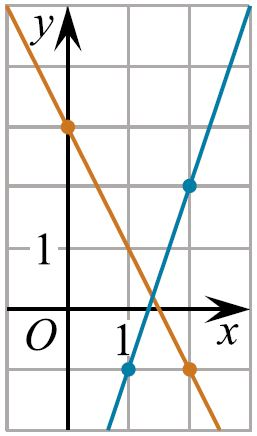
\includegraphics[align=t, width=0.8\textwidth]{../\picpath/G112M3C2-2}
		\end{minipage}
		\item
		\begin{minipage}[t]{\bodywidth}
			На рисунке изображён график функции вида \(f(x)=ax^2+bx+c\), где числа \(a, b, c\) --- целые. Найдите значение \(f(-3)\).
		\end{minipage}
		\begin{minipage}[t]{\picwidth}
			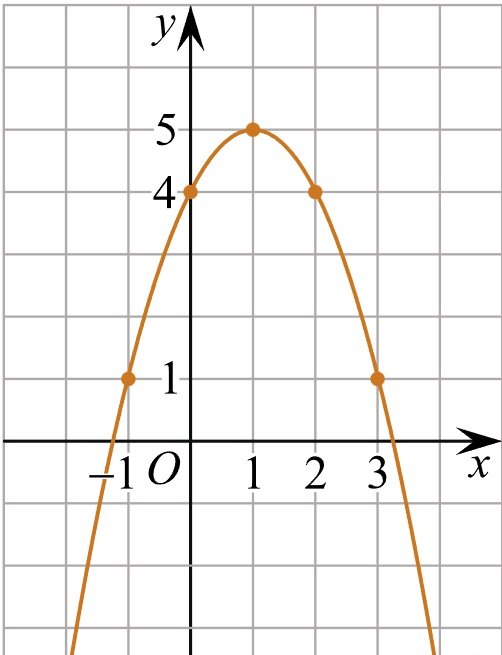
\includegraphics[align=t, width=\textwidth]{../\picpath/G101M4C4-3.jpg}
		\end{minipage}
		
		\item
		\begin{minipage}[t]{\bodywidth}
			На рисунке изображен график функции \( f(x)=\dfrac{x^2}{a}+bx+c \). Найдите \( f(3,5) \).
		\end{minipage}
		\begin{minipage}[t]{\picwidth}
			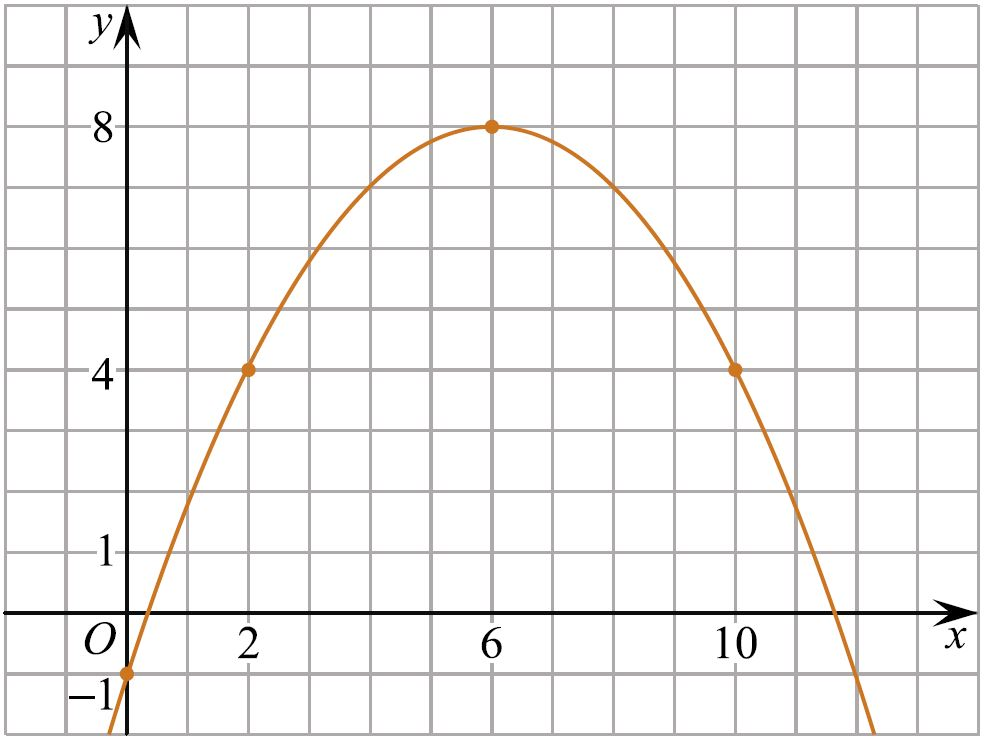
\includegraphics[align=t, width=\textwidth]{../\picpath/G112M3C2-3}
		\end{minipage}
		
		\item
		\begin{minipage}[t]{\bodywidth}
			На рисунке изображён график функции вида \(f(x)=ax^2+bx+c\), где числа \(a, b, c\) --- целые. Найдите значение дискриминанта уравнения \(f(x)=0\).
		\end{minipage}
		\begin{minipage}[t]{\picwidth}
			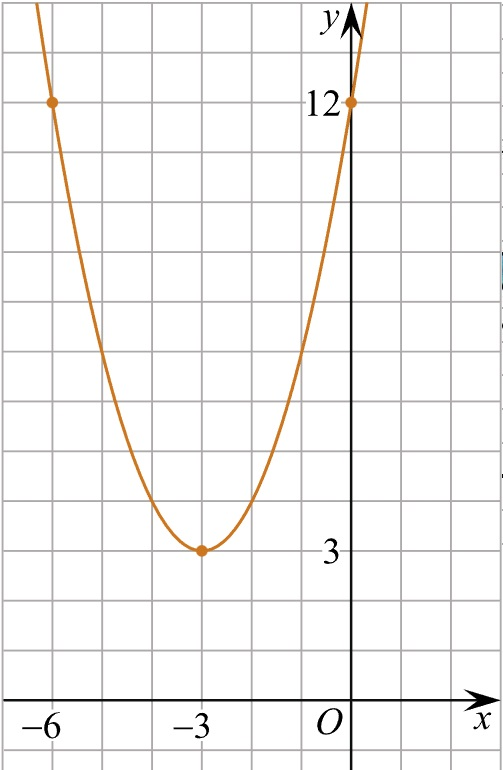
\includegraphics[align=t, width=\textwidth]{../\picpath/G101M4C4-5.jpg}
		\end{minipage}
		
		\item
		\begin{minipage}[t]{\bodywidth}
			На рисунке изображены графики функций \( f(x)=2x^2+11x+11 \) и \( y=ax^2+bx+c \), которые пересекаются в точках \( A \) и \( B \). Найдите абсциссу точки \( B \).
		\end{minipage}
		\begin{minipage}[t]{\picwidth}
			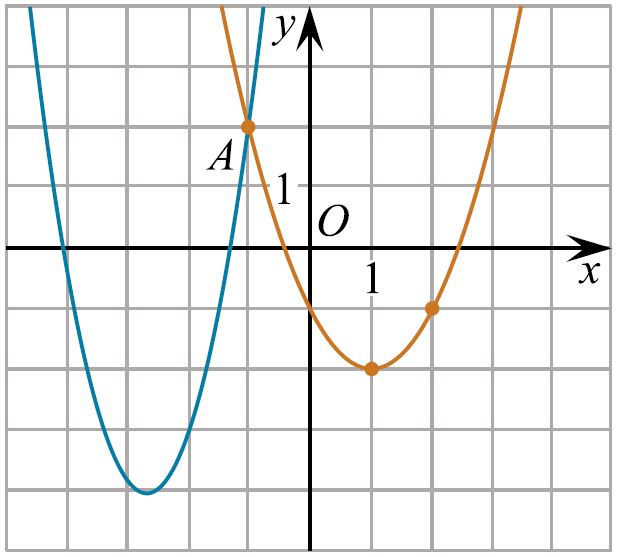
\includegraphics[align=t, width=\textwidth]{../\picpath/G112M3C2-6}
		\end{minipage}
		\item
		\begin{minipage}[t]{\bodywidth}
			На рисунке изображен график функции \( f(x)=\dfrac{k}{x}+a \). Найдите, при каком значении \( x \) значение функции будет равно \( 0,8 \).
		\end{minipage}
		\begin{minipage}[t]{\picwidth}
			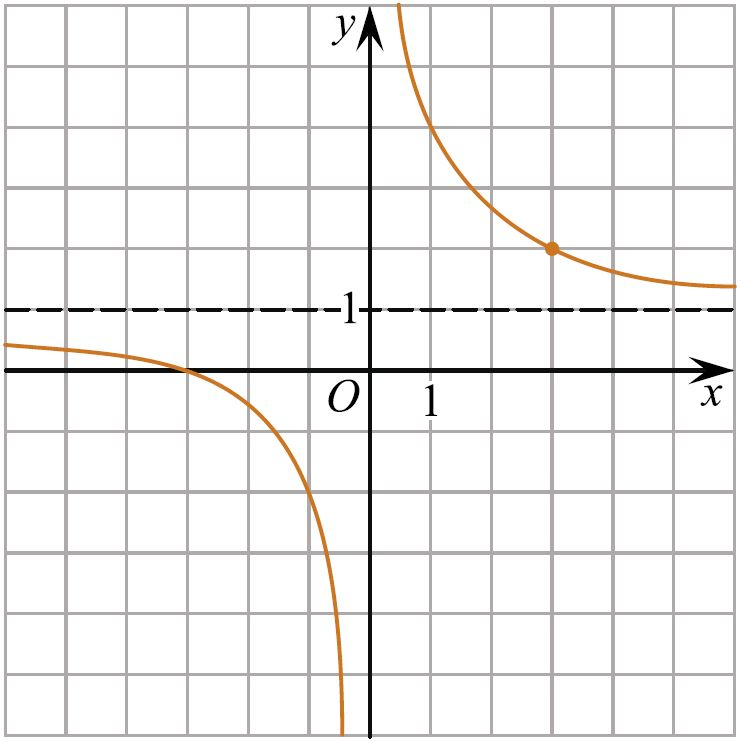
\includegraphics[align=t, width=\textwidth]{../\picpath/G112M3C2-5}
		\end{minipage}
		\item
		\begin{minipage}[t]{\bodywidth}
			На рисунке изображён график функции вида \[ f(x)=\dfrac{a}{x+b}+c, \] где числа \(a, b, c\) --- целые. Найдите значение \(x\), при котором \(f(x)=3\).
		\end{minipage}
		\hspace{0.02\linewidth}
		\begin{minipage}[t]{\picwidth}
			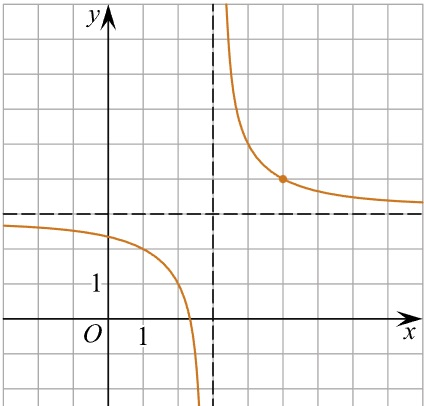
\includegraphics[align=t, width=\linewidth]{../\picpath/G101M4C6-2}
		\end{minipage}
		\newpage
		%analog 26784 1-2 V 62785 1-2
		\item Найдите:
		\begin{tasks}
			\task \( 8 \sin \left( \dfrac{ \pi }{ 2 }- \alpha \right) \), если \( \sin \alpha = -0,6 \) и \( \alpha \in (1,5\pi;2\pi) \);
			\task \( -2 \sin \left( \dfrac{ \pi }{ 2 }+\alpha \right) \), если \( \sin \alpha = -0,96 \) и \( \alpha \in (\pi;1,5\pi) \);
			\task \( -20 \cos \left( \dfrac{ 5\pi }{ 2 }+ \alpha \right) \), если \( \cos \alpha = \dfrac{ 7 }{ 25 } \) и \( \alpha \in (1,5\pi; 2\pi) \);
			\task \( 39 \cos \left( \dfrac{ 7\pi }{ 2 } + \alpha \right) \), если \( \cos \alpha = -\dfrac{ 7\pi }{ 2 } + \alpha \) и \( \alpha \in (0,5\pi;\pi) \).
		\end{tasks}
		\item Вычислите:
		\begin{tasks}(2)
			\task \( \dfrac{ 36 \sin 102 \degree \cdot \cos 102 \degree }{ \sin 204 \degree } \)
			\task \( \dfrac{ 50 \sin 38 \degree }{ \sin 19 \degree \cdot \cos 19 \degree } \)
			\task \( \dfrac{ -10 \sin 97 \degree \cdot \cos 97 \degree }{ \sin 194 \degree } \)
			\task \( \dfrac{ -16 \sin 112 \degree \cdot \cos 112 \degree }{ 5 \sin 224 \degree } \)
			\task \( \dfrac{22 (\sin^2 72 \degree - \cos^2 72 \degree)}{ \cos 144 \degree } \)
			\task \( \dfrac{ 22 \cos 18 \degree }{ \sin^2 9 \degree - \cos^2 9 \degree  } \)
			\task \( \dfrac{ 18(-\sin^2 24 \degree + \cos^2 24 \degree) }{ \cos 48 \degree } \)
			\task \( \dfrac{ 7(\sin^2 11 \degree - \cos^2 11 \degree) }{ -\cos 22 \degree } \)
		\end{tasks}
	\end{listofex}
\end{class}
%END_FOLD


%BEGIN_FOLD % ====>>_ Проверочная работа _<<====
\begin{exam}
	\begin{listofex}
		\item Проверочная
	\end{listofex}
\end{exam}
%END_FOLD